\section{Mjukvara}
\label{sec:Funktionalitet}
Mjukvaran som utvecklades består av tre olika system; en applikation som körs på
Fjärrkontrollen, en applikation som körs på Routern och ett program som körs på
ADKn. Androidapplikationerna är utvecklade i Java och behandlas i de första av
de kommande underavdelningarna.

Följande undersektioner kommer först behandla mjukvaruutvecklingen på de två
Androidapplikationerna för att sedan avsluta med utvecklingen gjord för ADKn.

\subsection{Fördelar vid Androidutveckling}
Ur en ekonomisk aspekt är det väldigt trevligt att jobba med utveckling av
Androidapplikationer, både utvecklingsvertyget Android SDK och utvecklingsmiljön
Eclipse är gratis. Dessutom så är Java språket, som Eclipse är skrivet i samt
språket man skriver Androidapplikationer i, plattformsoberoende.

Om man utgår från designmönstret Model-View-Controller \cite{MVC} så är
strukturen på de utvecklade applikationerna att Androidkomponenten Activity
\cite[Activity]{Android Reference} använd som en hybrid av Controller och View
och komponenten Service\cite[Service]{Android Reference} tillsammans med
ordinära javaklasser använda som Modeller.

\subsection{Fjärrkontroll}
Som nämnt i avsnitt \ref{subsec:system/fjarrkontroll} så har Fjärrkontrollen tre
stora uppgifter: generera styrsignaler till svävaren, kommunicera med de andra
enheterna samt att kunna logga händelser på svävaren.

Applikationen är uppdelad tre huvudsakliga delar som var och en utgörs av en
Android-service. Dessa delar implementerar funktionalitet för kommunikation,
loggning av sensordata samt generering av styrsignaler. Applikationen innehåller
även Android-activity som fungerar som inställningsmeny för fjärrkontrollen.

Genomgång på hur kommunikationen mellan fjärrkontrollen och de andra enheterna
sker gås igenom i avsnitt \ref{subsec:commlink} och generering av
styrsignaler behandlas i \ref{subsec:styr och regler}. Nedan beskrivs hur
loggning fungerar.

\subsubsection{Loggning av sensordata}
Funktionaliteten för att logga olika typer av sensordata sker genom att kryssa
i vilka sensorer som data ska sparas i från. Insamlade data sparas som textfiler
på fjärrkontrollens SD-minne.
På den senaste versionen av applikationen finns funktionalitet för loggning av
data från fjärrkontrollens accelerometer, svävarens accelerometer samt från
svävarens ultraljudssensorer. Vilken data som skall loggas ställs in i
inställningsmenyn. Om data från svävaren önskas skickas ett kommando till den
som gör att den svarar med ett paket innehållande önskad data.

\subsubsection{Resultat}
Fjärrkontrollen möter de krav som ställs i kravspecifikationen. Vid skrivandet
av rapporten hade tester dock bara genomförts på plattformar av
smartphone-modell.

\begin {itemize}
\item Räckvidd 20 meter
\item Indikera när kommunikationen med svävaren bryts.
\item Kunna kommunicera med svävaren. Samt ge de kommandon som gränssnittet till
svävaren tillåter.
\end {itemize}

\subsubsection{Vidareutveckling}
Som brukligt så blir man aldrig riktigt klar med utveckling av mjukvara, det
finns alltid saker att finslipa. Loggningsfunktionen bör kontrolleras noggrant
och utökas så att fler sensorer går att logga. Protocol Buffer är inte
implementerat som protokoll och det skulle med relativ enkelhet kunna ändras.

\subsection{Router}
Routerns uppgifter är att handha reglersystemet och att agera som
kommunikationslänk mellan de olika enheterna.

Programmet är indelat i tre Android-services och en Android-activity:
\begin{itemize}
	\item Bluetoothservice som hanterar all Bluetoothkommunkation,
	\item UsbService som hanterar all USBkommunkation,
	\item ControlSystemService som implementerar reglersystemet
	\item och MainActivity som implementerar användargränssnittet.
\end{itemize}

Applikationen startas automatiskt genom att ansluta ADK:n till router-telefonen. 
Om applikationen körs innan den ansluts till ADK:n kommer den att startas om för
att upprätta USB-kommunikationen.
När appen körs visas en diod för respektive kommunkationsbuss. Om kommunkationen
fungerar lyser dioden grönt och om den inte fungerar så lyser den rött. Dioden
kan även lysa gult men detta är inget man hinner se i vanliga fall då den enbart
gör så under uppkoppling. Knappen "Bluetooth setup" används för att upprätta en
Bluetoothlänk.

Intern kommunkation inom applikationen sker via Android Broadcasts.
Kommunikationen med andra enheter behandlas i avsnitt \ref{subsec:commlink} och
reglersystemet behandlas i \ref{subsec:styr och regler}.

\subsubsection{Resultat}
Programmet är stabilt och uppfyller alla krav. Dess huvudsyfte är att ta emot
och skicka vidare meddelanden vilket fungerar utmärkt.
\subsection{Kommunikationslank}
Mjukvarugänget\ldots
\subsubsection{Protocol buffer}
Protocol Buffer\cite{Protocol buffer} är ett protokoll som används för
serialisering av data.
Protokollet är utvecklat av Google, där Google har gjort kompilatorer för Java,
C++ och Python tillgängliga. Utöver dessa kompilatorer från Google så finns det
andra kompilatorer utvecklade av privatpersoner eller företag för andra språk.

Svävaren använder sig dels av Googles javakompilator för protokollet i 
fjärrkontrollen samt telefonen. För ADK:n så används en simplare version av
Protocol Buffer nämligen Nanopb \cite{Nanopb} som implementerar protokollet i
statisk C kod.

Det Protocol Buffer generar är programkod med funktionalitet för att kunna
serialisera och deserialisera olika dataobjekt. Dessa dataobjekt beskrivs av
användaren med ett IDL (Interface Definition Language).
Svävaren använder sig av sju stycken olika dataobjekt för sin kommunikation(se
appendix xxx fil Command.proto).

\subsubsection{ADK till Telefon}
Rickard och Jens\ldots
\subsubsection{Telefon till fjärrkontroll}
Johan\ldots

\subsection{Styr- och reglersystem}
\label{subsec:styr och regler}
För att styra svävaren samlas acclerometerdata in i realtid på fjärrkontrollen som sedan processeras och omvandlas till styrsignaler som skickas till routern där det även finns plats för ett reglersystem.

\subsubsection{Styrsystem}
Det finns tre olika styralgorithmer för att processera pitch- och rolldata separat. De tre olika styralgorithmerna processerar acclerometerdatan på liknande sätt men med olika matamatiska funktioner, de tre lägena är logaritmisk, exponentionell och linjär. Man kan genom dropdown listor på fjärrkontrollen välja vilken styralgoritm som ska användas. De olika styralgoritmerna utvecklades med hjälp av MATLAB för att sedan implementeras i JAVA på fjärrkontrollen. De olika styralgoritmernas utslag då pitch = 30\degree  då roll går från -45\degree till 45\degree  kan ses i figur~\ref{fig:styralgoritmer}.

\begin{figure}[htbp!]
\centering
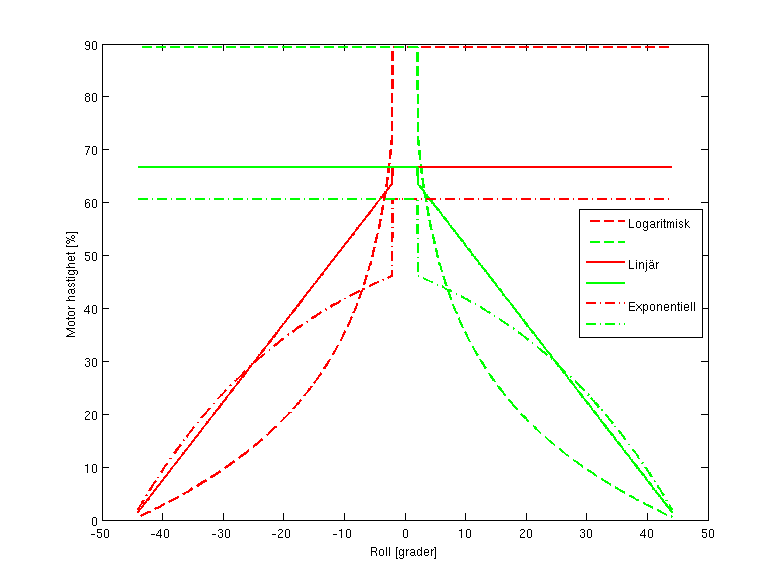
\includegraphics[width=12cm]{../../includes/figures/Styralgoritmer}
\caption{Styralgoritmernas utslag vid pitch = 30\degree då roll = [-45,45].}
\label{fig:styralgoritmer}
\end{figure}

I realiteten märkte föraren dock ingen större skillnad mellan de olika styrlägena. 

\subsubsection{Reglersystem}
Designen av svävaren medförde att hastighet och styrning var starkt korskopplade vilket medför svårigheter då en regulator ska implementeras. Grundlig efterforskning gjordes och det bestämdes att ramverket ACADO skulle användas för att implementera en regulator till svävaren då ramverket kunde autogenerera kod för mer komplexa regulatorer. Detta visade sig vara svårare än förutspått och ramverket krävde även mer minne än vad som fanns tillgängligt. Dessa bakslag medförde att reglersystemet lades på is för att kunna vidareutvecklas vid ett senare tillfälle.

\subsection{ADK}
ADK:n ansvarar för att skicka styrsignaler till motorer och fläktar och hantera sensorer på svävaren. 
Den kommunicerar med routern via USB.

För att få en bättre kodstruktur på C-koden togs beslutet att ett realtids operativsystem (RTOS) 
eller eventsystem skulle användas.

Flera färdiga kodbibliotek användes i arbetet med ADK:n. 

\begin{table}[htb]
\centering
\caption{Bibliotek som används på ADK:n}
\label{tbl:BOM}
\begin{tabular}{|l|p{0.5\textwidth}|c|}
\hline
\textbf{Namn} & \textbf{Information} & \textbf{Referens} \\
\hline
Arduino Core & Stöd för Arduinos funktioner. Krävs för att arbeta med Arduino i Eclipse &  \cite{Delta_BFB1212VH-R00}\\ 
\hline
USB\_Host & Sköter USB kommunikation och tillhandahåller enkla läs och skrivfunktioner för USB & \cite{USBHost}\\
\hline
Wire & Standardbibliotek för Arduino som sköter I2C kommunikation &  \cite{Wire}\\
\hline
Event System & Ett simpelt event system anpassat för Arduino & \cite{Eventsystem} \\
\hline
\end{tabular}	
\end{table}

\subsubsection{Resultat}
USB länken har under tester varit stabil.
Kommunikationen består av protocollbuffer meddelanden.

ADKn styr svävaren genom att tolka och vidarebefordra styrsignalerna 
som den får från fjärrkontrollen till svävarens motorer och fläktar. 
Förutom att hantera styrsignaler kan ADKn ta in sensordata från de fyra ultraljuds 
sensorerna som finns på svävaren och med hjälp av dessa få fram avstånd till objekt framför och bakom svävaren.
Det finns även kod som sköter inläsning av kompassdata från en elektronisk kompass [XXXXX] via I2C men den 
används ej då kompassen inte behövdes i den slutgiltiga versionen.

Efter en undersökning om vilka alternativ som fanns tillgängliga av eventsystem och RTOS togs beslutet 
att använda ett eventsystem då de RTOS som hittades var mer komplicerade än vad som behövdes för detta projekt.
Det eventsystem som används är enkelt att använda och utifrån de tester som utförts verkar det stabilt vid normal drift. 
Detta medför att det blir enkelt att som programmerare lägga till till nya events på ADKn och 
vara säker på att dessa hanteras. 
Dock upptäcktes det svagheter i eventsystemet vid stresstest, dvs då man ökar hur ofta den ska behandla events. 
Det berodde på att ADKn inte hann utföra alla events och man kunde då inte längre lita på att alla events utfördes.

\subsubsection{Diskussion}
ADKn utför sin uppgift på ett tillfredsställande sätt. 
Det finns dock flera svagheter som går att förbättra om vidareutveckling skulle ske.
Ett exempel är eventsystemet, det är simpelt vilket innebär att det är lätt att sätta sig in i och använda men det
har stabilitetsproblem om man ökar antalet events eller hur ofta de sker. Det skulle kunna förbättras genom att ändra i 
den kod som används idag, hitta ett annat eventsystem eller kanske framförallt byta till ett fungerande RTOS. 
Ett RTOS skulle öka stabiliteten och man skulle kunna öka antalet parallella aktiviter men skulle ta mycket tid att 
förstå och få att fungera.

Om mer tid och pengar funnits hade det även varit intressant att använda sig av sensorer med stöd för I2C för avståndsberäkning. 
Det skulle innebära att färre pinnar på ADKn skulle användas och leda till en estetiskt mer tilltalande koppling. 
Det skulle även vara intressant att öka antalet sensorer så att man kan få in mer sensordata, t.ex. kompass eller gps-data.
\subsection{Sensorer}
Rickard och Emil\ldots